\documentclass{beamer}
\usepackage{graphicx}
\usepackage{longtable}
\usepackage{pdflscape} 
\usepackage{rotating}
\usepackage{tabularray}
\usepackage{siunitx}
\UseTblrLibrary{siunitx}
\UseTblrLibrary{booktabs}
\usepackage{colortbl}
\usepackage{xcolor}

\mode<presentation>
{
	\usetheme{Szeged}      % or try Darmstadt, Madrid, Warsaw, ...
	\usecolortheme{seahorse} % or try albatross, beaver, crane, ...
	\usefonttheme{serif}  % or try serif, structurebold, ...
	\setbeamertemplate{navigation symbols}{}
	\setbeamertemplate{caption}[numbered]
} 

\usepackage[english]{babel}
\usepackage[utf8x]{inputenc}
\title[Replication Project]{Replication Project}
\author{Rosalie LaCroix}
\institute{Applied Stats II}
\date{03/04/2026}

\begin{document}
	
	\begin{frame}
		\titlepage
	\end{frame}
	
	% Uncomment these lines for an automatically generated outline.
	%\begin{frame}{Outline}
	%  \tableofcontents
	%\end{frame}
	
	\section{Original Study}
	
	\begin{frame}{Who Shot the Bullets? Exposure to Violence and Attitudes Toward Peace: Evidence from the 2016 Colombian Referendum}
		Kreiman, G., \& Masullo, J. (2020). Who Shot the Bullets? Exposure to Violence and Attitudes Toward Peace: Evidence from the 2016 Colombian Referendum. Latin American Politics and Society, 62(4), 24–49. doi:10.1017/lap.2020.14
	\end{frame}
	
	\begin{frame}{Historical Context}
		\begin{itemize}
			\item Colombian Conflict
				\item FARC, paramilitaries, BACRIM
			\item Election of Juan Manuel Santos and Peace Talks
			\item 2016 Peace Referendum
		\end{itemize}	
	\end{frame}
	
	\begin{frame}{Research Question and Hypotheses}
		\textbf{Question:} Does variation in experiences of violence also translate into different attitudes toward peace? Specifically, investigates whether exposure to violence by the FARC, as opposed to violence by the paramilitaries and BACRIM, had an observable impact on vote choice.
		
		\textbf{Hypotheses:}
		
		\begin{itemize}
			\item In areas where Group A has committed most of the violence, residents are more likely to support a peace agreement with Group A.
			\item In areas where Group B has committed most of the violence, residents are less likely to support a peace agreement with Group A.
		\end{itemize}
	\end{frame}
	
	\section{Data}
	
	\begin{frame}{Model and Variables}
		\begin{itemize}
			\item \textbf{OLS Model}
		\end{itemize}
			\textbf{Dependent Variable:}
		\begin{itemize}
			\item \% of votes per municipality supporting the 2016 peace agreement referendum
		\end{itemize}
		
		\textbf{Independent Variables:}
		
		\noindent Set of variables measuring the average number of violent attacks carried out by FARC and paramilitaries/BACRIM from the years 1988-2010.
		\begin{itemize}
			\item (ln) FARC attacks (ln\_atfarc\_cede)
			\item (ln) Paramilitary/BACRIM attacks (ln\_atparabacrim\_cede)
		\end{itemize}
		
	\end{frame}
	
	\begin{frame}{Control Variables included in Regression}
			\noindent Set of variables included in their models that could have an impact on perceived violence and voting in referendum 
		\begin{itemize}
			\item \% Votes for Santos in 2014 Election (ref\_partic)
			\item \% Participation in Referendum (share\_santos\_2\_100)
			\item Poverty Measure (incidence\_multidim\_pov\_2005\_100)
			\item Population Measure (lpop)
			\item Rurality Index (indrural2005)
			\item Coca Cultivation (cultivated100)
			\item Oil Present (oil)
			\item Elevation (ln\_altitud)
			\item Education (coberturabrutaeduc)
		\end{itemize}
	\end{frame}
	
	\begin{frame}{Departmental Fixed Effects}
			\textbf{Fixed Effects Model}
		\begin{itemize}
			\item Control for unobserved characteristics that do not change over time and are specific to each department
			\item 32 departments and 1 capital district
		\end{itemize}
	\end{frame}
	
	\section{Replication}
	
	\begin{frame}{Table 1. OLS Identity Perpetrator (Models 5-7)}
	\begin{table}
		\centering
		\scalebox{0.60}{
			\begin{tblr}[         %% tabularray outer open
				caption={OLS Identity Perpetrator (Models 5--7)},
				note{}={* p \num{< 0.1}, ** p \num{< 0.05}, *** p \num{< 0.01}},
				]                     %% tabularray outer close
				{                     %% tabularray inner open
					colspec={Q[]Q[]Q[]Q[]},
					row{2}={bg=yellow!30},
					row{4}={bg=yellow!30},
					hline{2}={1-4}{solid, black, 0.05em},
					hline{27}={1-4}{solid, black, 0.05em},
					hline{1}={1-4}{solid, black, 0.08em},
					hline{30}={1-4}{solid, black, 0.08em},
					column{2-4}={}{halign=c},
					column{1}={}{halign=l},
				}                     %% tabularray inner close
				& (5) & (6) & (7) \\
				(ln) FARC attacks & \num{1.100}*** & \num{1.050}*** & \num{1.058}*** \\
				& (\num{0.249}) & (\num{0.254}) & (\num{0.264}) \\
				(ln) Paramilitary/BACRIM attacks & \num{-1.608}*** & \num{-1.470}*** & \num{-1.322}*** \\
				& (\num{0.418}) & (\num{0.431}) & (\num{0.445}) \\
				\% Support Santos 2014 & \num{0.596}*** & \num{0.589}*** & \num{0.585}*** \\
				& (\num{0.022}) & (\num{0.023}) & (\num{0.025}) \\
				Rural Index & \num{0.092}*** & \num{0.083}*** & \num{0.085}*** \\
				& (\num{0.021}) & (\num{0.022}) & (\num{0.023}) \\
				Coca &  & \num{2.022}** & \num{2.128}** \\
				&  & (\num{1.028}) & (\num{1.039}) \\
				Oil &  & \num{-1.627} & \num{-1.781}* \\
				&  & (\num{1.036}) & (\num{1.047}) \\
				Department Fixed Effects & $\checkmark$ & $\checkmark$ & $\checkmark$ \\
				Constant & \num{30.221}** & \num{20.008}*** & \num{18.778}* \\
				& (\num{12.045}) & (\num{7.414}) & (\num{9.602}) \\
				Num.Obs. & \num{927} & \num{887} & \num{857} \\
				R2 & \num{0.720} & \num{0.710} & \num{0.699} \\
				R2 Adj. & \num{0.708} & \num{0.698} & \num{0.685} \\
			\end{tblr}
		}
	\end{table}
	\end{frame}
	
	\begin{frame}{Figure 1. Exposure to Violence and Vote Choices in the Referendum}
		\begin{figure}[htbp]
			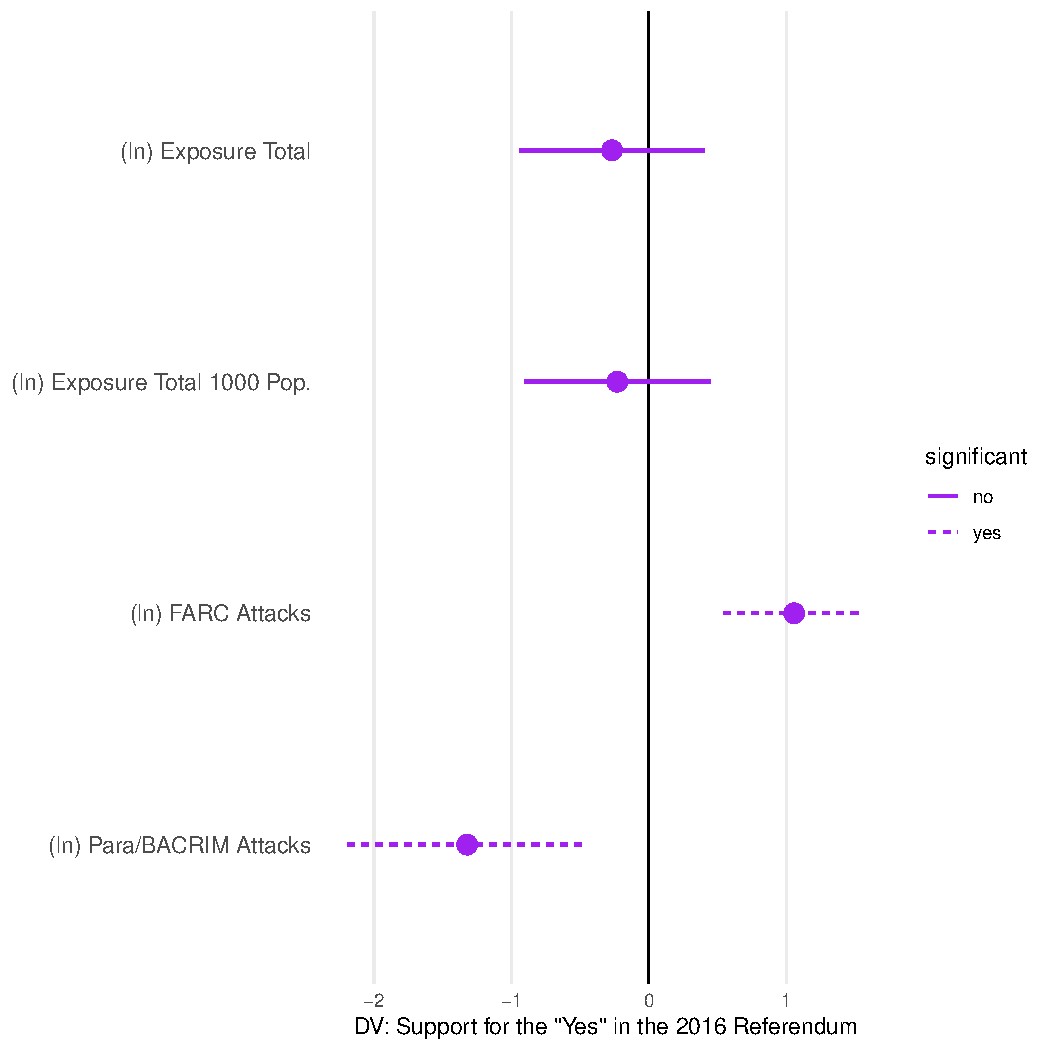
\includegraphics[width=\linewidth, height=0.75\textheight, keepaspectratio]{figure_1.pdf}
		\end{figure}
	\end{frame}
	
	\begin{frame}{Interpreting Results and Findings}
		\textbf{Table 1:}
		\begin{itemize}
			\item \small Holding all other variables constant, on average, for every one percent increase in the mean number of FARC attacks in a municipality, the percentage of votes per municipality supporting the 2016 peace agreement referendum increases by .01058\%.
			\item \small Holding all other variables constant, on average, for every one percent increase in the mean number of Para/BACRIM attacks in a municipality, the percentage of votes per municipality supporting the 2016 peace agreement referendum decreases by .01322\%.
		\end{itemize}
		\textbf{Figure 1:}
		\begin{itemize}
			\item \small "Overall levels of violent attacks by all armed groups in each Colombian municipality do not have an impact on citizens' support for the peace agreement, clear (and statistically significant) effects emerge when we disaggregate by the identity of the perpetrator."
		\end{itemize}
	\end{frame}
	
	\begin{frame}{Problems with Replication}
		\begin{itemize}
			\item Authors did not use a uniform reference category
			\item Some departments had a very small number of municipalities within them
			\item Authors had an incorrect interpretation of their regression coefficients
		\end{itemize}
		
	\end{frame}
	
	\section{My Contribution}
	
	\begin{frame}{My Contribution: Multilevel Model}
		\begin{itemize}
			\item Extension of linear regression, but allows for more accurate inferences for grouped data by allowing the intercept, or both the intercept and slopes, to vary
			\item Group and individual level variation is considered within the estimation of the group-level coefficients
			\item In between no pooling and full pooling 	\footnote{Gelman \& Hill (2018)}
		\end{itemize}
	
	\end{frame}
	
	\begin{frame}{Multilevel Model Setup}
		\begin{figure}
			\includegraphics[width=0.7\linewidth]{"Screenshot 2026-03-30 at 12.01.42.pdf"}
		\end{figure}
		\begin{figure}
			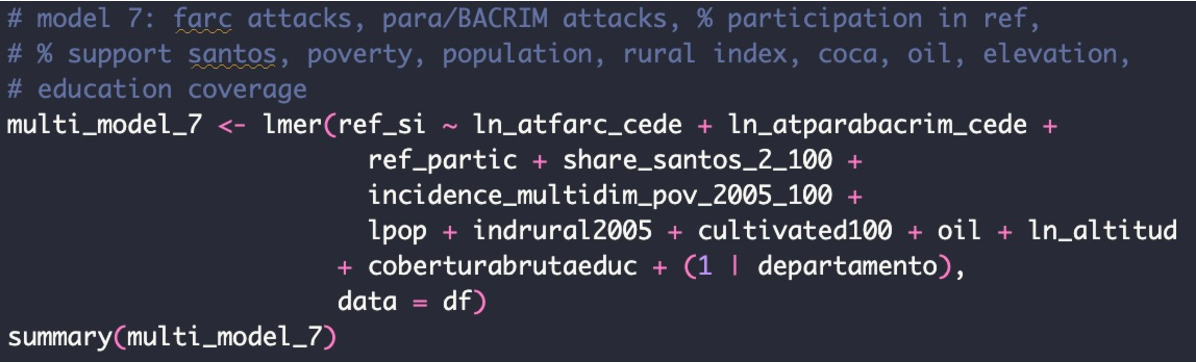
\includegraphics[width=0.7\linewidth]{Screenshot 2026-03-30 at 12.02.00.pdf}
		\end{figure}
	\end{frame}

	\begin{frame}{Table 2. Multilevel Model Results}
		\centering
		\scalebox{0.60}{
		\begin{tabular}{l c c c}
			\toprule
			& Model 5 & Model 6 & Model 7 \\
			\midrule
			\rowcolor{purple!30}
			(Intercept)                         & $15.63^{*}$   & $18.26^{**}$  & $20.16^{*}$  \\
	    	& $(6.66)$      & $(6.88)$      & $(8.46)$     \\
			\rowcolor{yellow!30}
			ln\_atfarc\_cede                    & $1.05^{***}$  & $0.98^{***}$  & $1.03^{***}$ \\
			& $(0.24)$      & $(0.25)$      & $(0.26)$     \\
			\rowcolor{yellow!30}
			ln\_atparabacrim\_cede              & $-1.67^{***}$ & $-1.45^{***}$ & $-1.34^{**}$ \\
		 	& $(0.41)$      & $(0.42)$      & $(0.44)$     \\
			share\_santos\_2\_100         & $0.60^{***}$  & $0.59^{***}$  & $0.58^{***}$ \\
		 	& $(0.02)$      & $(0.02)$      & $(0.02)$     \\
			indrural2005   & $0.09^{***}$  & $0.08^{***}$  & $0.08^{***}$ \\
			& $(0.02)$      & $(0.02)$      & $(0.02)$     \\
			Num. obs.                           & $927$         & $887$         & $857$        \\
			Num. groups: departamento            & $33$          & $27$          & $26$         \\
			Var: departamento (Intercept)       & $19.71$       & $19.02$       & $19.47$      \\
			Var: Residual                      & $78.73$       & $79.81$       & $79.97$      \\
			\bottomrule
			\multicolumn{4}{l}{\scriptsize{$^{***}p<0.001$; $^{**}p<0.01$; $^{*}p<0.05$}}
		\end{tabular}
	}
	\end{frame}
	
	\begin{frame}[fragile=singleslide]{Multilevel Model Intercepts}
		\begin{figure}
			\includegraphics[width=0.7\linewidth]{"Screenshot 2026-03-30 at 12.03.36.pdf"}
		\end{figure}
		\textbf{Output:}
		\begin{verbatim}
			Intercept.
			departamento_10     24.27479
			departamento_11     21.28139
			departamento_12     17.28407
		\end{verbatim}
			\textbf{departamento\_10}: The average expected value of the percentage of votes per municipality within department 10 supporting the 2016 peace agreement referendum, when all covariates are 0 is 24.27\%.	

	\end{frame}
	
	\begin{frame}{Understanding the Incorrect Interpretation}
		\begin{figure}
			\includegraphics[width=0.7\linewidth]{"Screenshot 2026-03-30 at 13.15.29.pdf"}
		\end{figure}
		
		\textbf{Author's Interpretation:}
		"If the mean of FARC attacks in a given municipality increases by 1\%, the yes vote in the referendum increases by approximately 1.06 points."
		
		\begin{itemize}
			\item They cannot make this claim about their outcome variable
			\item Why?
		\end{itemize}
		
	\end{frame}
	
	\begin{frame}{Predicted Probabilities}
		In order to understand if this claim was correct and how/why they could be making it, I chose to determine predicted probabilities of \% yes votes in referendum for varying numbers of FARC attacks and para/BACRIM attacks, and subsequently plot these values against the exponentiated (ln) FARC Attacks and (ln) Para/BACRIM Attacks variable values to get the true raw counts.
		
	\end{frame}
	
	\begin{frame}{Predicted Probabilities}
		\centering
		\includegraphics[width=0.7\linewidth]{"Screenshot 2026-03-30 at 13.32.59.pdf"}
		\includegraphics[width=0.7\linewidth]{"Screenshot 2026-03-30 at 13.33.13.pdf"}
	\end{frame}	
	
	\begin{frame}{FARC Attack Counts vs Predicted Probabilities of \% Yes Votes in Referendum}
		\begin{figure}
			\centering
			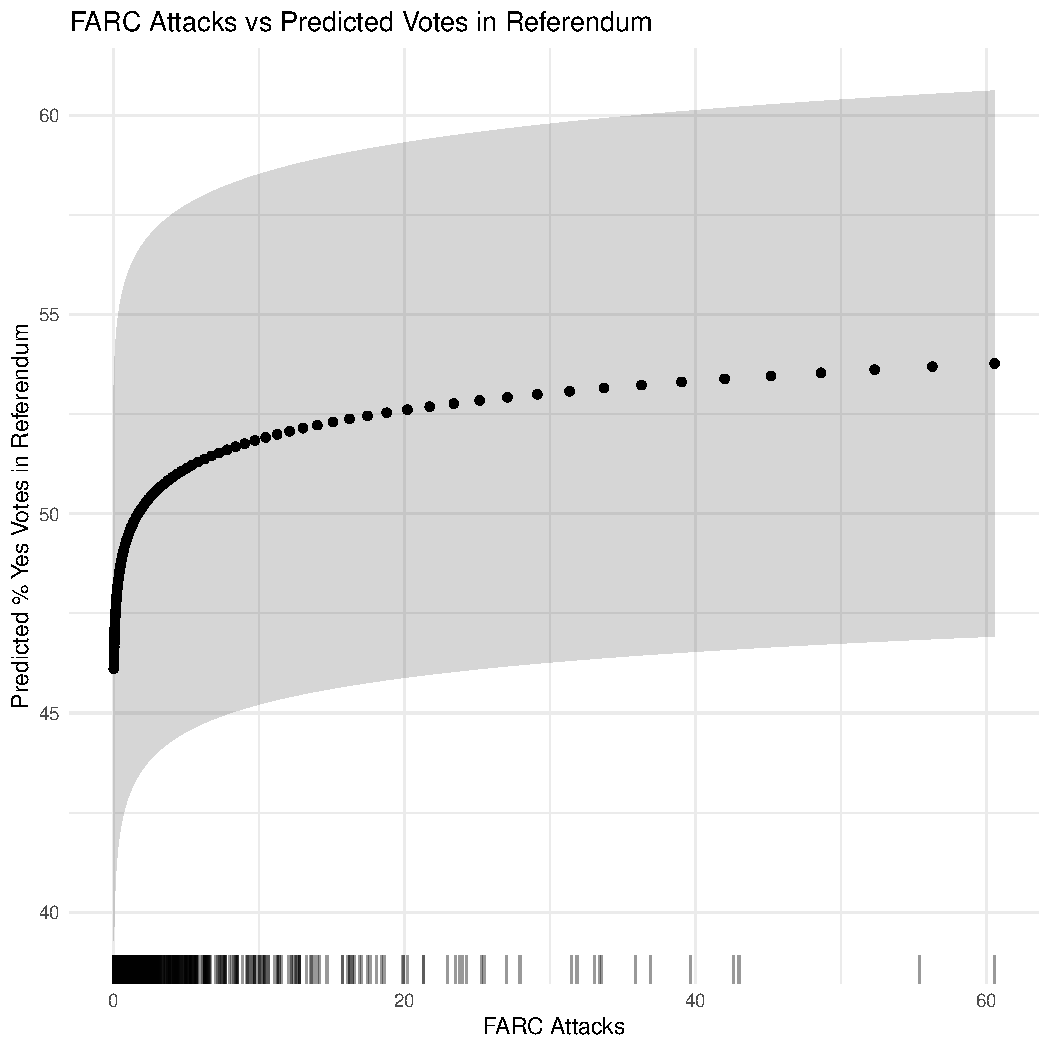
\includegraphics[width=\linewidth, height=0.75\textheight, keepaspectratio]{pred_plot.pdf}
		\end{figure}
	\end{frame}		
	\begin{frame}{Para/BACRIM Attack Counts vs Predicted Probabilities of \% Yes Votes in Referendum}
		\begin{figure}
			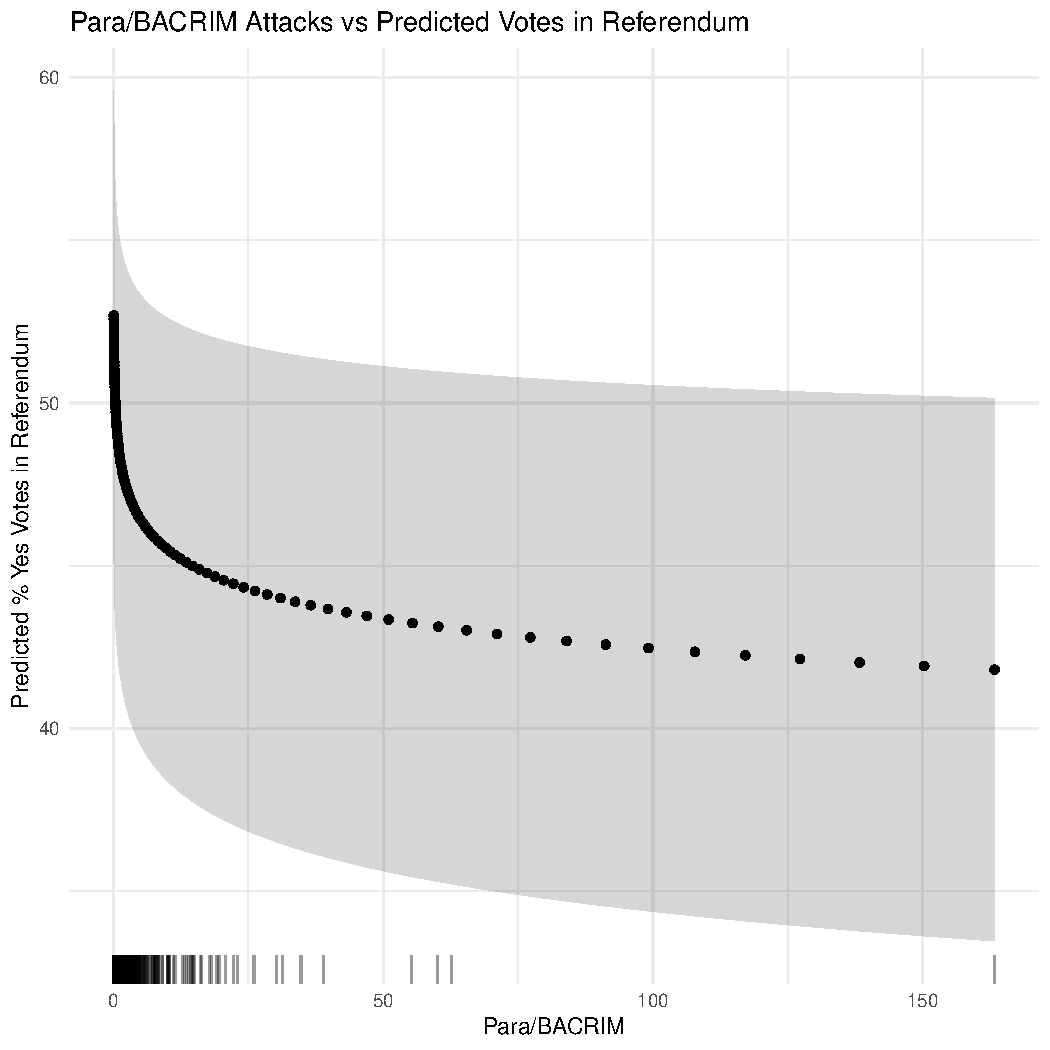
\includegraphics[width=\linewidth, height=0.75\textheight, keepaspectratio]{pred_plot_para.pdf}
		\end{figure}
	\end{frame}
	
	\begin{frame}{What this Means}
			The author's interpretation is wrong, the correct interpretation is:
		
			\textbf{FARC Attacks:} Holding all other variables constant, for every 1\% increase in the mean count of FARC attacks in a given municipality, the yes vote in the referendum increases by approximately 0.0106 points.
			
			\textbf{Para/BACRIM Attacks:} Holding all other variables constant, for every 1\% increase in the mean count of para/BACRIM attacks in a given municipality, the yes vote in the referendum decreases by approximately 0.0132 points.
		
	\end{frame}
	
	\section{References}
	
	\begin{frame}{References}
	
	Gelman, A., \& Hill, J. (2018). \textit{Data analysis using regression and multilevel/hierarchical models}. Cambridge University Press.
	
	\vspace{0.2cm}
	
	Clark, M. (n.d.). \textit{Models demystified -- Michael Clark}. Github.io. 
	Retrieved March 25, 2026, from https://m-clark.github.io/category=mixed\%20models
	
	\end{frame}
	
\end{document}
